\documentclass[onecolumn]{article}
%\usepackage{url}
%\usepackage{algorithmic}
\usepackage[a4paper]{geometry}
\usepackage{datetime}
\usepackage[margin=2em, font=small,labelfont=it]{caption}
\usepackage{graphicx}
\usepackage{mathpazo} % use palatino
\usepackage[scaled]{helvet} % helvetica
\usepackage{microtype}
\usepackage{amsmath}
\usepackage{subfigure}
% Letterspacing macros
\newcommand{\spacecaps}[1]{\textls[200]{\MakeUppercase{#1}}}
\newcommand{\spacesc}[1]{\textls[50]{\textsc{\MakeLowercase{#1}}}}

\title{\spacecaps{Project module report: Argumentation Mining }\\ \normalsize \spacesc{University of Potsdam, Winter semester 2017/18} }

\author{Oğuz Serbetci\\Maria Stazherova}
%\date{\today\\\currenttime}
\date{\today}

\begin{document}
\maketitle

\begin{abstract}

Maybe just short description of the task and results here

\end{abstract}


\section{Data \& Task}
We worked with the arg-microtext corpus \cite{peldszus2015annotated}, which contains 112 short argumentative texts 
(originally in German and profesionally translated to English). Later we received preliminary annotations of the new microtexts
and could incorporate them into the project.

\begin{figure}[h]
    \centering
    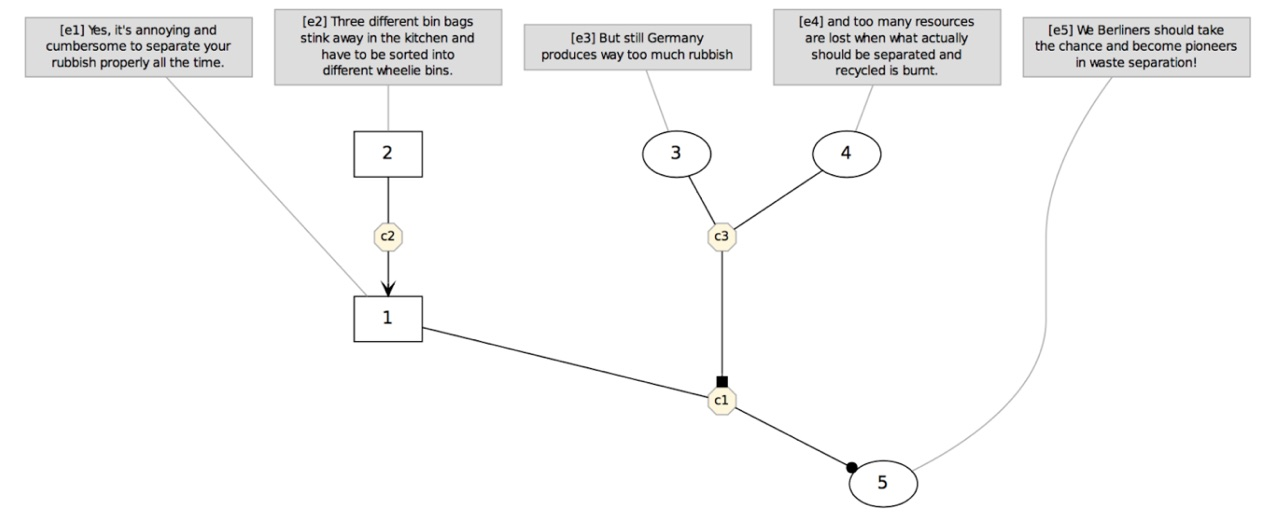
\includegraphics[width=\linewidth]{fig/microtext.jpg}
    \caption{One example from arg-microtext corpus and its argumentation graph.
            \\Round nodes are proponent's nodes, square ones are opponent's nodes. The arcs connecting the nodes represent different supporting and attacking moves.}
    \label{fig:microtext}
        \end{figure}

As can be seen in the figure \ref{fig:microtext}, each text in the corpus is a single tree and argument components (ACs) are claims and premises.  
We decided to concentrate on two tasks: classify the type of an AC (claim or premise), and determining the links between ACs.

\section{Approach}
Here we could try describing the workflow

\subsection{Challenges}
encountered difficulties and how they were solved 



\section{Results}

Here go the final results

\section{Conclusion}
like future work ideas?

\nocite{*}
\bibliographystyle{plain}
\bibliography{references}
\end{document}
